\documentclass[11pt,compress,t,notes=noshow, xcolor=table]{beamer}

\documentclass[11pt,compress,t,notes=noshow, xcolor=table]{beamer}
\usepackage[]{graphicx}\usepackage[]{color}
% maxwidth is the original width if it is less than linewidth
% otherwise use linewidth (to make sure the graphics do not exceed the margin)
\makeatletter
\def\maxwidth{ %
  \ifdim\Gin@nat@width>\linewidth
    \linewidth
  \else
    \Gin@nat@width
  \fi
}
\makeatother

\definecolor{fgcolor}{rgb}{0.345, 0.345, 0.345}
\newcommand{\hlnum}[1]{\textcolor[rgb]{0.686,0.059,0.569}{#1}}%
\newcommand{\hlstr}[1]{\textcolor[rgb]{0.192,0.494,0.8}{#1}}%
\newcommand{\hlcom}[1]{\textcolor[rgb]{0.678,0.584,0.686}{\textit{#1}}}%
\newcommand{\hlopt}[1]{\textcolor[rgb]{0,0,0}{#1}}%
\newcommand{\hlstd}[1]{\textcolor[rgb]{0.345,0.345,0.345}{#1}}%
\newcommand{\hlkwa}[1]{\textcolor[rgb]{0.161,0.373,0.58}{\textbf{#1}}}%
\newcommand{\hlkwb}[1]{\textcolor[rgb]{0.69,0.353,0.396}{#1}}%
\newcommand{\hlkwc}[1]{\textcolor[rgb]{0.333,0.667,0.333}{#1}}%
\newcommand{\hlkwd}[1]{\textcolor[rgb]{0.737,0.353,0.396}{\textbf{#1}}}%
\let\hlipl\hlkwb

\usepackage{framed}
\makeatletter
\newenvironment{kframe}{%
 \def\at@end@of@kframe{}%
 \ifinner\ifhmode%
  \def\at@end@of@kframe{\end{minipage}}%
  \begin{minipage}{\columnwidth}%
 \fi\fi%
 \def\FrameCommand##1{\hskip\@totalleftmargin \hskip-\fboxsep
 \colorbox{shadecolor}{##1}\hskip-\fboxsep
     % There is no \\@totalrightmargin, so:
     \hskip-\linewidth \hskip-\@totalleftmargin \hskip\columnwidth}%
 \MakeFramed {\advance\hsize-\width
   \@totalleftmargin\z@ \linewidth\hsize
   \@setminipage}}%
 {\par\unskip\endMakeFramed%
 \at@end@of@kframe}
\makeatother

\definecolor{shadecolor}{rgb}{.97, .97, .97}
\definecolor{messagecolor}{rgb}{0, 0, 0}
\definecolor{warningcolor}{rgb}{1, 0, 1}
\definecolor{errorcolor}{rgb}{1, 0, 0}
\newenvironment{knitrout}{}{} % an empty environment to be redefined in TeX

\usepackage{alltt}
\newcommand{\SweaveOpts}[1]{}  % do not interfere with LaTeX
\newcommand{\SweaveInput}[1]{} % because they are not real TeX commands
\newcommand{\Sexpr}[1]{}       % will only be parsed by R
\newcommand{\xmark}{\ding{55}}%


\usepackage[english]{babel}
\usepackage[utf8]{inputenc}

\usepackage{dsfont}
\usepackage{verbatim}
\usepackage{amsmath}
\usepackage{amsfonts}
\usepackage{amssymb}
\usepackage{bm}
\usepackage{csquotes}
\usepackage{multirow}
\usepackage{longtable}
\usepackage{booktabs}
\usepackage{enumerate}
\usepackage[absolute,overlay]{textpos}
\usepackage{psfrag}
\usepackage{algorithm}
\usepackage{algpseudocode}
\usepackage{eqnarray}
\usepackage{arydshln}
\usepackage{tabularx}
\usepackage{placeins}
\usepackage{tikz}
\usepackage{setspace}
\usepackage{colortbl}
\usepackage{mathtools}
\usepackage{wrapfig}
\usepackage{bm}
\usepackage{amsmath}
\usepackage{pifont}

\usetikzlibrary{shapes,arrows,automata,positioning,calc,chains,trees, shadows}
\tikzset{
  %Define standard arrow tip
  >=stealth',
  %Define style for boxes
  punkt/.style={
    rectangle,
    rounded corners,
    draw=black, very thick,
    text width=6.5em,
    minimum height=2em,
    text centered},
  % Define arrow style
  pil/.style={
    ->,
    thick,
    shorten <=2pt,
    shorten >=2pt,}
}

\usepackage{subfig}

% Defines macros and environments
\usepackage{../../style/lmu-lecture}


\let\code=\texttt
\let\proglang=\textsf

\setkeys{Gin}{width=0.9\textwidth}

\setbeamertemplate{frametitle}{\expandafter\uppercase\expandafter\insertframetitle}

\usepackage{bbm}
% basic latex stuff
\newcommand{\pkg}[1]{{\fontseries{b}\selectfont #1}} %fontstyle for R packages
\newcommand{\lz}{\vspace{0.5cm}} %vertical space
\newcommand{\dlz}{\vspace{1cm}} %double vertical space
\newcommand{\oneliner}[1] % Oneliner for important statements
{\begin{block}{}\begin{center}\begin{Large}#1\end{Large}\end{center}\end{block}}


%new environments
\newenvironment{vbframe}  %frame with breaks and verbatim
{
 \begin{frame}[containsverbatim,allowframebreaks]
}
{
\end{frame}
}

\newenvironment{vframe}  %frame with verbatim without breaks (to avoid numbering one slided frames)
{
 \begin{frame}[containsverbatim]
}
{
\end{frame}
}

\newenvironment{blocki}[1]   % itemize block
{
 \begin{block}{#1}\begin{itemize}
}
{
\end{itemize}\end{block}
}

\newenvironment{fragileframe}[2]{  %fragile frame with framebreaks
\begin{frame}[allowframebreaks, fragile, environment = fragileframe]
\frametitle{#1}
#2}
{\end{frame}}


\newcommand{\myframe}[2]{  %short for frame with framebreaks
\begin{frame}[allowframebreaks]
\frametitle{#1}
#2
\end{frame}}

\newcommand{\remark}[1]{
  \textbf{Remark:} #1
}


\newenvironment{deleteframe}
{
\begingroup
\usebackgroundtemplate{
\includegraphics[width=\paperwidth,height=\paperheight]{../style/color/red.png}}
 \begin{frame}
}
{
\end{frame}
\endgroup
}
\newenvironment{simplifyframe}
{
\begingroup
\usebackgroundtemplate{
\includegraphics[width=\paperwidth,height=\paperheight]{../style/color/yellow.png}}
 \begin{frame}
}
{
\end{frame}
\endgroup
}\newenvironment{draftframe}
{
\begingroup
\usebackgroundtemplate{
\includegraphics[width=\paperwidth,height=\paperheight]{../style/color/green.jpg}}
 \begin{frame}
}
{
\end{frame}
\endgroup
}
% https://tex.stackexchange.com/a/261480: textcolor that works in mathmode
\makeatletter
\renewcommand*{\@textcolor}[3]{%
  \protect\leavevmode
  \begingroup
    \color#1{#2}#3%
  \endgroup
}
\makeatother





% math spaces
\ifdefined\N                                                                
\renewcommand{\N}{\mathds{N}} % N, naturals
\else \newcommand{\N}{\mathds{N}} \fi 
\newcommand{\Z}{\mathds{Z}} % Z, integers
\newcommand{\Q}{\mathds{Q}} % Q, rationals
\newcommand{\R}{\mathds{R}} % R, reals
\ifdefined\C 
  \renewcommand{\C}{\mathds{C}} % C, complex
\else \newcommand{\C}{\mathds{C}} \fi
\newcommand{\continuous}{\mathcal{C}} % C, space of continuous functions
\newcommand{\M}{\mathcal{M}} % machine numbers
\newcommand{\epsm}{\epsilon_m} % maximum error

% counting / finite sets
\newcommand{\setzo}{\{0, 1\}} % set 0, 1
\newcommand{\setmp}{\{-1, +1\}} % set -1, 1
\newcommand{\unitint}{[0, 1]} % unit interval

% basic math stuff
\newcommand{\xt}{\tilde x} % x tilde
\newcommand{\argmax}{\operatorname{arg\,max}} % argmax
\newcommand{\argmin}{\operatorname{arg\,min}} % argmin
\newcommand{\argminlim}{\mathop{\mathrm{arg\,min}}\limits} % argmax with limits
\newcommand{\argmaxlim}{\mathop{\mathrm{arg\,max}}\limits} % argmin with limits  
\newcommand{\sign}{\operatorname{sign}} % sign, signum
\newcommand{\I}{\mathbb{I}} % I, indicator
\newcommand{\order}{\mathcal{O}} % O, order
\newcommand{\pd}[2]{\frac{\partial{#1}}{\partial #2}} % partial derivative
\newcommand{\floorlr}[1]{\left\lfloor #1 \right\rfloor} % floor
\newcommand{\ceillr}[1]{\left\lceil #1 \right\rceil} % ceiling

% sums and products
\newcommand{\sumin}{\sum\limits_{i=1}^n} % summation from i=1 to n
\newcommand{\sumim}{\sum\limits_{i=1}^m} % summation from i=1 to m
\newcommand{\sumjn}{\sum\limits_{j=1}^n} % summation from j=1 to p
\newcommand{\sumjp}{\sum\limits_{j=1}^p} % summation from j=1 to p
\newcommand{\sumik}{\sum\limits_{i=1}^k} % summation from i=1 to k
\newcommand{\sumkg}{\sum\limits_{k=1}^g} % summation from k=1 to g
\newcommand{\sumjg}{\sum\limits_{j=1}^g} % summation from j=1 to g
\newcommand{\meanin}{\frac{1}{n} \sum\limits_{i=1}^n} % mean from i=1 to n
\newcommand{\meanim}{\frac{1}{m} \sum\limits_{i=1}^m} % mean from i=1 to n
\newcommand{\meankg}{\frac{1}{g} \sum\limits_{k=1}^g} % mean from k=1 to g
\newcommand{\prodin}{\prod\limits_{i=1}^n} % product from i=1 to n
\newcommand{\prodkg}{\prod\limits_{k=1}^g} % product from k=1 to g
\newcommand{\prodjp}{\prod\limits_{j=1}^p} % product from j=1 to p

% linear algebra
\newcommand{\one}{\boldsymbol{1}} % 1, unitvector
\newcommand{\zero}{\mathbf{0}} % 0-vector
\newcommand{\id}{\boldsymbol{I}} % I, identity
\newcommand{\diag}{\operatorname{diag}} % diag, diagonal
\newcommand{\trace}{\operatorname{tr}} % tr, trace
\newcommand{\spn}{\operatorname{span}} % span
\newcommand{\scp}[2]{\left\langle #1, #2 \right\rangle} % <.,.>, scalarproduct
\newcommand{\mat}[1]{\begin{pmatrix} #1 \end{pmatrix}} % short pmatrix command
\newcommand{\Amat}{\mathbf{A}} % matrix A
\newcommand{\Deltab}{\mathbf{\Delta}} % error term for vectors

% basic probability + stats
\renewcommand{\P}{\mathds{P}} % P, probability
\newcommand{\E}{\mathds{E}} % E, expectation
\newcommand{\var}{\mathsf{Var}} % Var, variance
\newcommand{\cov}{\mathsf{Cov}} % Cov, covariance
\newcommand{\corr}{\mathsf{Corr}} % Corr, correlation
\newcommand{\normal}{\mathcal{N}} % N of the normal distribution
\newcommand{\iid}{\overset{i.i.d}{\sim}} % dist with i.i.d superscript
\newcommand{\distas}[1]{\overset{#1}{\sim}} % ... is distributed as ...

% machine learning
\newcommand{\Xspace}{\mathcal{X}} % X, input space
\newcommand{\Yspace}{\mathcal{Y}} % Y, output space
\newcommand{\nset}{\{1, \ldots, n\}} % set from 1 to n
\newcommand{\pset}{\{1, \ldots, p\}} % set from 1 to p
\newcommand{\gset}{\{1, \ldots, g\}} % set from 1 to g
\newcommand{\Pxy}{\mathbb{P}_{xy}} % P_xy
\newcommand{\Exy}{\mathbb{E}_{xy}} % E_xy: Expectation over random variables xy
\newcommand{\xv}{\mathbf{x}} % vector x (bold)
\newcommand{\xtil}{\tilde{\mathbf{x}}} % vector x-tilde (bold)
\newcommand{\yv}{\mathbf{y}} % vector y (bold)
\newcommand{\xy}{(\xv, y)} % observation (x, y)
\newcommand{\xvec}{\left(x_1, \ldots, x_p\right)^\top} % (x1, ..., xp) 
\newcommand{\Xmat}{\mathbf{X}} % Design matrix
\newcommand{\allDatasets}{\mathds{D}} % The set of all datasets
\newcommand{\allDatasetsn}{\mathds{D}_n}  % The set of all datasets of size n 
\newcommand{\D}{\mathcal{D}} % D, data
\newcommand{\Dn}{\D_n} % D_n, data of size n
\newcommand{\Dtrain}{\mathcal{D}_{\text{train}}} % D_train, training set
\newcommand{\Dtest}{\mathcal{D}_{\text{test}}} % D_test, test set
\newcommand{\xyi}[1][i]{\left(\xv^{(#1)}, y^{(#1)}\right)} % (x^i, y^i), i-th observation
\newcommand{\Dset}{\left( \xyi[1], \ldots, \xyi[n]\right)} % {(x1,y1)), ..., (xn,yn)}, data
\newcommand{\defAllDatasetsn}{(\Xspace \times \Yspace)^n} % Def. of the set of all datasets of size n 
\newcommand{\defAllDatasets}{\bigcup_{n \in \N}(\Xspace \times \Yspace)^n} % Def. of the set of all datasets 
\newcommand{\xdat}{\left\{ \xv^{(1)}, \ldots, \xv^{(n)}\right\}} % {x1, ..., xn}, input data
\newcommand{\ydat}{\left\{ \yv^{(1)}, \ldots, \yv^{(n)}\right\}} % {y1, ..., yn}, input data
\newcommand{\yvec}{\left(y^{(1)}, \hdots, y^{(n)}\right)^\top} % (y1, ..., yn), vector of outcomes
\renewcommand{\xi}[1][i]{\xv^{(#1)}} % x^i, i-th observed value of x
\newcommand{\yi}[1][i]{y^{(#1)}} % y^i, i-th observed value of y 
\newcommand{\xivec}{\left(x^{(i)}_1, \ldots, x^{(i)}_p\right)^\top} % (x1^i, ..., xp^i), i-th observation vector
\newcommand{\xj}{\xv_j} % x_j, j-th feature
\newcommand{\xjvec}{\left(x^{(1)}_j, \ldots, x^{(n)}_j\right)^\top} % (x^1_j, ..., x^n_j), j-th feature vector
\newcommand{\phiv}{\mathbf{\phi}} % Basis transformation function phi
\newcommand{\phixi}{\mathbf{\phi}^{(i)}} % Basis transformation of xi: phi^i := phi(xi)

%%%%%% ml - models general
\newcommand{\lamv}{\bm{\lambda}} % lambda vector, hyperconfiguration vector
\newcommand{\Lam}{\bm{\Lambda}}	 % Lambda, space of all hpos
% Inducer / Inducing algorithm
\newcommand{\preimageInducer}{\left(\defAllDatasets\right)\times\Lam} % Set of all datasets times the hyperparameter space
\newcommand{\preimageInducerShort}{\allDatasets\times\Lam} % Set of all datasets times the hyperparameter space
% Inducer / Inducing algorithm
\newcommand{\ind}{\mathcal{I}} % Inducer, inducing algorithm, learning algorithm 

% continuous prediction function f
\newcommand{\ftrue}{f_{\text{true}}}  % True underlying function (if a statistical model is assumed)
\newcommand{\ftruex}{\ftrue(\xv)} % True underlying function (if a statistical model is assumed)
\newcommand{\fx}{f(\xv)} % f(x), continuous prediction function
\newcommand{\fdomains}{f: \Xspace \rightarrow \R^g} % f with domain and co-domain
\newcommand{\Hspace}{\mathcal{H}} % hypothesis space where f is from
\newcommand{\fbayes}{f^{\ast}} % Bayes-optimal model
\newcommand{\fxbayes}{f^{\ast}(\xv)} % Bayes-optimal model
\newcommand{\fkx}[1][k]{f_{#1}(\xv)} % f_j(x), discriminant component function
\newcommand{\fh}{\hat{f}} % f hat, estimated prediction function
\newcommand{\fxh}{\fh(\xv)} % fhat(x)
\newcommand{\fxt}{f(\xv ~|~ \thetab)} % f(x | theta)
\newcommand{\fxi}{f\left(\xv^{(i)}\right)} % f(x^(i))
\newcommand{\fxih}{\hat{f}\left(\xv^{(i)}\right)} % f(x^(i))
\newcommand{\fxit}{f\left(\xv^{(i)} ~|~ \thetab\right)} % f(x^(i) | theta)
\newcommand{\fhD}{\fh_{\D}} % fhat_D, estimate of f based on D
\newcommand{\fhDtrain}{\fh_{\Dtrain}} % fhat_Dtrain, estimate of f based on D
\newcommand{\fhDnlam}{\fh_{\Dn, \lamv}} %model learned on Dn with hp lambda
\newcommand{\fhDlam}{\fh_{\D, \lamv}} %model learned on D with hp lambda
\newcommand{\fhDnlams}{\fh_{\Dn, \lamv^\ast}} %model learned on Dn with optimal hp lambda 
\newcommand{\fhDlams}{\fh_{\D, \lamv^\ast}} %model learned on D with optimal hp lambda 

% discrete prediction function h
\newcommand{\hx}{h(\xv)} % h(x), discrete prediction function
\newcommand{\hh}{\hat{h}} % h hat
\newcommand{\hxh}{\hat{h}(\xv)} % hhat(x)
\newcommand{\hxt}{h(\xv | \thetab)} % h(x | theta)
\newcommand{\hxi}{h\left(\xi\right)} % h(x^(i))
\newcommand{\hxit}{h\left(\xi ~|~ \thetab\right)} % h(x^(i) | theta)
\newcommand{\hbayes}{h^{\ast}} % Bayes-optimal classification model
\newcommand{\hxbayes}{h^{\ast}(\xv)} % Bayes-optimal classification model

% yhat
\newcommand{\yh}{\hat{y}} % yhat for prediction of target
\newcommand{\yih}{\hat{y}^{(i)}} % yhat^(i) for prediction of ith targiet
\newcommand{\resi}{\yi- \yih}

% theta
\newcommand{\thetah}{\hat{\theta}} % theta hat
\newcommand{\thetab}{\bm{\theta}} % theta vector
\newcommand{\thetabh}{\bm{\hat\theta}} % theta vector hat
\newcommand{\thetat}[1][t]{\thetab^{[#1]}} % theta^[t] in optimization
\newcommand{\thetatn}[1][t]{\thetab^{[#1 +1]}} % theta^[t+1] in optimization
\newcommand{\thetahDnlam}{\thetabh_{\Dn, \lamv}} %theta learned on Dn with hp lambda
\newcommand{\thetahDlam}{\thetabh_{\D, \lamv}} %theta learned on D with hp lambda
\newcommand{\mint}{\min_{\thetab \in \Theta}} % min problem theta
\newcommand{\argmint}{\argmin_{\thetab \in \Theta}} % argmin theta

% densities + probabilities
% pdf of x 
\newcommand{\pdf}{p} % p
\newcommand{\pdfx}{p(\xv)} % p(x)
\newcommand{\pixt}{\pi(\xv~|~ \thetab)} % pi(x|theta), pdf of x given theta
\newcommand{\pixit}[1][i]{\pi\left(\xi[#1] ~|~ \thetab\right)} % pi(x^i|theta), pdf of x given theta
\newcommand{\pixii}[1][i]{\pi\left(\xi[#1]\right)} % pi(x^i), pdf of i-th x 

% pdf of (x, y)
\newcommand{\pdfxy}{p(\xv,y)} % p(x, y)
\newcommand{\pdfxyt}{p(\xv, y ~|~ \thetab)} % p(x, y | theta)
\newcommand{\pdfxyit}{p\left(\xi, \yi ~|~ \thetab\right)} % p(x^(i), y^(i) | theta)

% pdf of x given y
\newcommand{\pdfxyk}[1][k]{p(\xv | y= #1)} % p(x | y = k)
\newcommand{\lpdfxyk}[1][k]{\log p(\xv | y= #1)} % log p(x | y = k)
\newcommand{\pdfxiyk}[1][k]{p\left(\xi | y= #1 \right)} % p(x^i | y = k)

% prior probabilities
\newcommand{\pik}[1][k]{\pi_{#1}} % pi_k, prior
\newcommand{\lpik}[1][k]{\log \pi_{#1}} % log pi_k, log of the prior
\newcommand{\pit}{\pi(\thetab)} % Prior probability of parameter theta

% posterior probabilities
\newcommand{\post}{\P(y = 1 ~|~ \xv)} % P(y = 1 | x), post. prob for y=1
\newcommand{\postk}[1][k]{\P(y = #1 ~|~ \xv)} % P(y = k | y), post. prob for y=k
\newcommand{\pidomains}{\pi: \Xspace \rightarrow \unitint} % pi with domain and co-domain
\newcommand{\pibayes}{\pi^{\ast}} % Bayes-optimal classification model
\newcommand{\pixbayes}{\pi^{\ast}(\xv)} % Bayes-optimal classification model
\newcommand{\pix}{\pi(\xv)} % pi(x), P(y = 1 | x)
\newcommand{\piv}{\bm{\pi}} % pi, bold, as vector
\newcommand{\pikx}[1][k]{\pi_{#1}(\xv)} % pi_k(x), P(y = k | x)
\newcommand{\pikxt}[1][k]{\pi_{#1}(\xv ~|~ \thetab)} % pi_k(x | theta), P(y = k | x, theta)
\newcommand{\pixh}{\hat \pi(\xv)} % pi(x) hat, P(y = 1 | x) hat
\newcommand{\pikxh}[1][k]{\hat \pi_{#1}(\xv)} % pi_k(x) hat, P(y = k | x) hat
\newcommand{\pixih}{\hat \pi(\xi)} % pi(x^(i)) with hat
\newcommand{\pikxih}[1][k]{\hat \pi_{#1}(\xi)} % pi_k(x^(i)) with hat
\newcommand{\pdfygxt}{p(y ~|~\xv, \thetab)} % p(y | x, theta)
\newcommand{\pdfyigxit}{p\left(\yi ~|~\xi, \thetab\right)} % p(y^i |x^i, theta)
\newcommand{\lpdfygxt}{\log \pdfygxt } % log p(y | x, theta)
\newcommand{\lpdfyigxit}{\log \pdfyigxit} % log p(y^i |x^i, theta)

% probababilistic
\newcommand{\bayesrulek}[1][k]{\frac{\P(\xv | y= #1) \P(y= #1)}{\P(\xv)}} % Bayes rule
\newcommand{\muk}{\bm{\mu_k}} % mean vector of class-k Gaussian (discr analysis) 

% residual and margin
\newcommand{\eps}{\epsilon} % residual, stochastic
\newcommand{\epsi}{\epsilon^{(i)}} % epsilon^i, residual, stochastic
\newcommand{\epsh}{\hat{\epsilon}} % residual, estimated
\newcommand{\yf}{y \fx} % y f(x), margin
\newcommand{\yfi}{\yi \fxi} % y^i f(x^i), margin
\newcommand{\Sigmah}{\hat \Sigma} % estimated covariance matrix
\newcommand{\Sigmahj}{\hat \Sigma_j} % estimated covariance matrix for the j-th class

% ml - loss, risk, likelihood
\newcommand{\Lyf}{L\left(y, f\right)} % L(y, f), loss function
\newcommand{\Lypi}{L\left(y, \pi\right)} % L(y, pi), loss function
\newcommand{\Lxy}{L\left(y, \fx\right)} % L(y, f(x)), loss function
\newcommand{\Lxyi}{L\left(\yi, \fxi\right)} % loss of observation
\newcommand{\Lxyt}{L\left(y, \fxt\right)} % loss with f parameterized
\newcommand{\Lxyit}{L\left(\yi, \fxit\right)} % loss of observation with f parameterized
\newcommand{\Lxym}{L\left(\yi, f\left(\bm{\tilde{x}}^{(i)} ~|~ \thetab\right)\right)} % loss of observation with f parameterized
\newcommand{\Lpixy}{L\left(y, \pix\right)} % loss in classification
\newcommand{\Lpiv}{L\left(y, \piv\right)} % loss in classification
\newcommand{\Lpixyi}{L\left(\yi, \pixii\right)} % loss of observation in classification
\newcommand{\Lpixyt}{L\left(y, \pixt\right)} % loss with pi parameterized
\newcommand{\Lpixyit}{L\left(\yi, \pixit\right)} % loss of observation with pi parameterized
\newcommand{\Lhxy}{L\left(y, \hx\right)} % L(y, h(x)), loss function on discrete classes
\newcommand{\Lr}{L\left(r\right)} % L(r), loss defined on residual (reg) / margin (classif)
\newcommand{\lone}{|y - \fx|} % L1 loss
\newcommand{\ltwo}{\left(y - \fx\right)^2} % L2 loss
\newcommand{\lbernoullimp}{\ln(1 + \exp(-y \cdot \fx))} % Bernoulli loss for -1, +1 encoding
\newcommand{\lbernoullizo}{- y \cdot \fx + \log(1 + \exp(\fx))} % Bernoulli loss for 0, 1 encoding
\newcommand{\lcrossent}{- y \log \left(\pix\right) - (1 - y) \log \left(1 - \pix\right)} % cross-entropy loss
\newcommand{\lbrier}{\left(\pix - y \right)^2} % Brier score
\newcommand{\risk}{\mathcal{R}} % R, risk
\newcommand{\riskbayes}{\mathcal{R}^\ast}
\newcommand{\riskf}{\risk(f)} % R(f), risk
\newcommand{\riskdef}{\E_{y|\xv}\left(\Lxy \right)} % risk def (expected loss)
\newcommand{\riskt}{\mathcal{R}(\thetab)} % R(theta), risk
\newcommand{\riske}{\mathcal{R}_{\text{emp}}} % R_emp, empirical risk w/o factor 1 / n
\newcommand{\riskeb}{\bar{\mathcal{R}}_{\text{emp}}} % R_emp, empirical risk w/ factor 1 / n
\newcommand{\riskef}{\riske(f)} % R_emp(f)
\newcommand{\risket}{\mathcal{R}_{\text{emp}}(\thetab)} % R_emp(theta)
\newcommand{\riskr}{\mathcal{R}_{\text{reg}}} % R_reg, regularized risk
\newcommand{\riskrt}{\mathcal{R}_{\text{reg}}(\thetab)} % R_reg(theta)
\newcommand{\riskrf}{\riskr(f)} % R_reg(f)
\newcommand{\riskrth}{\hat{\mathcal{R}}_{\text{reg}}(\thetab)} % hat R_reg(theta)
\newcommand{\risketh}{\hat{\mathcal{R}}_{\text{emp}}(\thetab)} % hat R_emp(theta)
\newcommand{\LL}{\mathcal{L}} % L, likelihood
\newcommand{\LLt}{\mathcal{L}(\thetab)} % L(theta), likelihood
\newcommand{\LLtx}{\mathcal{L}(\thetab | \xv)} % L(theta|x), likelihood
\newcommand{\logl}{\ell} % l, log-likelihood
\newcommand{\loglt}{\logl(\thetab)} % l(theta), log-likelihood
\newcommand{\logltx}{\logl(\thetab | \xv)} % l(theta|x), log-likelihood
\newcommand{\errtrain}{\text{err}_{\text{train}}} % training error
\newcommand{\errtest}{\text{err}_{\text{test}}} % test error
\newcommand{\errexp}{\overline{\text{err}_{\text{test}}}} % avg training error

% lm
\newcommand{\thx}{\thetab^\top \xv} % linear model
\newcommand{\olsest}{(\Xmat^\top \Xmat)^{-1} \Xmat^\top \yv} % OLS estimator in LM 



\newcommand{\titlefigure}{figure_man/convex_programs.png}
\newcommand{\learninggoals}{
\item Strategy
\item Basic Method
\item Updating
}


%\usepackage{animate} % only use if you want the animation for Taylor2D

\title{Optimization in Machine Learning}
%\author{Bernd Bischl}
\date{}

\begin{document}

\lecturechapter{CMA-ES Algorithm}
\lecture{Optimization in Machine Learning}
\sloppy
%%%%%%%%%%%%%%%%%%%%%%%%%%%%%%%%%%%%%%%%%%%%%%%%%%%%%%%%%%%%%%%%%%%%%%%%%%%%%%%%%%%

% \section{Covariance Matrix Adaptation Evolution Strategy (CMA-ES)}

%\begin{vbframe}{CMA-ES as part of many EDAs}
%\textbf{Estimation of Distribution Algorithms} (EDAs) widely used class of algorithms designed to solve optimization problems of the form
%
%\vspace{-10pt}
%\begin{eqnarray*}
%\xv^* = \argmax_{\xv \in \mathcal{S}} f(\xv), \quad \text{where } f:\mathcal{S}\rightarrow \R.
%\end{eqnarray*}
%
%
%Instead of solving above objective directly, EDAs solve related objective:
%\begin{eqnarray*}
%\thetab^\ast = \argmax_{\thetab} \E_{p(\xv|\thetab)} f(\xv),
%\end{eqnarray*}
%\vspace{-10pt}
%
%where $p(\xv|\thetab)$ is a probability density over $\mathcal{S}$, parameterized by $p$ parameters $\thetab \in \R^p$.
%
%\lz
%
%Reason for later formulation: convenience of derivative-free optimization, enabling of rigorous analysis and leveraging of a probabilistic formulation to incorporate auxiliary information.
%\end{vbframe}
%% \framebreak
\begin{frame}{CMA-ES}

\begin{minipage}{0.62\textwidth}
General algorithmic template with initial parameter setting $\bm{\theta}^{[0]}$ of parameterized density $p(\xv|\thetab)$, such that each iteration $t \in \{0,1,\dots, T\}$ consist of:

\begin{enumerate}
\item Draw $\lambda$ samples, $\xv^{(k)}$ from $p(\bm{x}|\thetab^{[t]})$
\item Evaluate $W(f(\xv^{(k)}))$, where $W(\cdot)$ gives weights for each $\xv^{(k)}$, typically $0$ or $1$ (order-preserving fitness transformation)
\item Find a $\thetab^{[t+1]}$ that uses weighted samples and corresponding function evaluations to move $p(\xv|\thetab)$ towards regions $\mathcal{S}$ that have large function values.
\end{enumerate}

%This core algorithm is often modified in a variety of ways to improve performance via \textbf{Covariance Matrix Adaptation (CMA-ES)}.
\end{minipage}\hfill
\begin{minipage}{0.35\textwidth}\raggedleft
\begin{figure}
  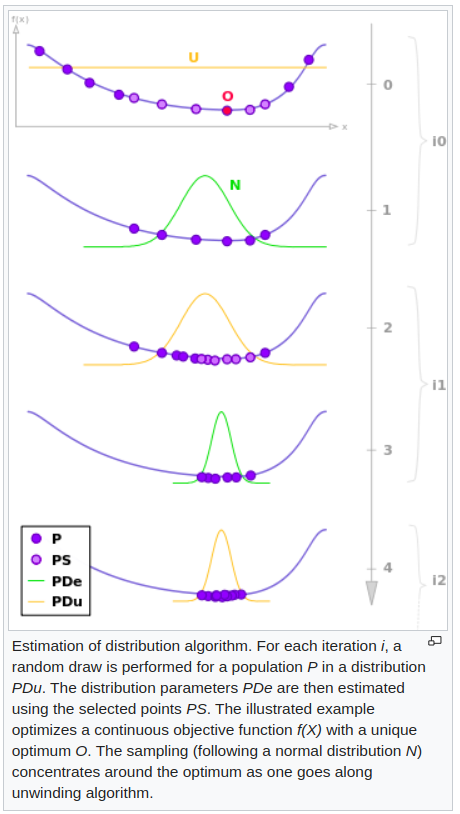
\includegraphics[width=1\textwidth, height=0.9\textheight]{figure_man/cmaes/cmaes_eda.png}
\end{figure}
\end{minipage}

\end{frame}


\begin{vbframe}{CMA-ES}

Covariance Matrix Adaptation Evolution Strategy (CMA-ES) is

\begin{itemize}
\item A state-of-the-art tool in evolutionary computation (derivative-free)
\item A stochastic/randomized method
\item For usage in continuous domain
\item For non-linear, non-convex optimization problems
\item Useful in case \enquote{classical} search methods like quasi-Newton methods (BFGS) or conjugate gradient methods fail due to a non-convex or rugged search landscape (e.g. outliers, noise, local optima, sharp bends).
\end{itemize}

Detailed information on CMA-ES can be found in

\begin{enumerate}
\item Nikolaus Hansen. The CMA Evolution Strategy. 2005
\item A. Auger, N. Hansen: Tutorial CMA-ES: Evolution Strategies and Covariance Matrix Adaptation. 2012.
\end{enumerate}

\end{vbframe}


\begin{vbframe}{CMA-ES: Strategy}
A population of new search points (individuals, offspring) is generated by sampling a multivariate normal distribution. A repeated update of the mean vector and covariance matrix with the respectively best ranked individuals moves the distributions towards the optimum.

Search points for generation number $t = 0, 1, \dots, T$:

\vspace{-10pt}

\begin{eqnarray*}
\xv^{[t+1](k)} \sim \bm{m}^{[t]} + \sigma^{[t]} \normal (\bm{0}, \bm{C}^{[t]}) \quad \text{for } k = 1, \dots, \lambda.
\end{eqnarray*}
\vspace{-20pt}

\begin{figure}
  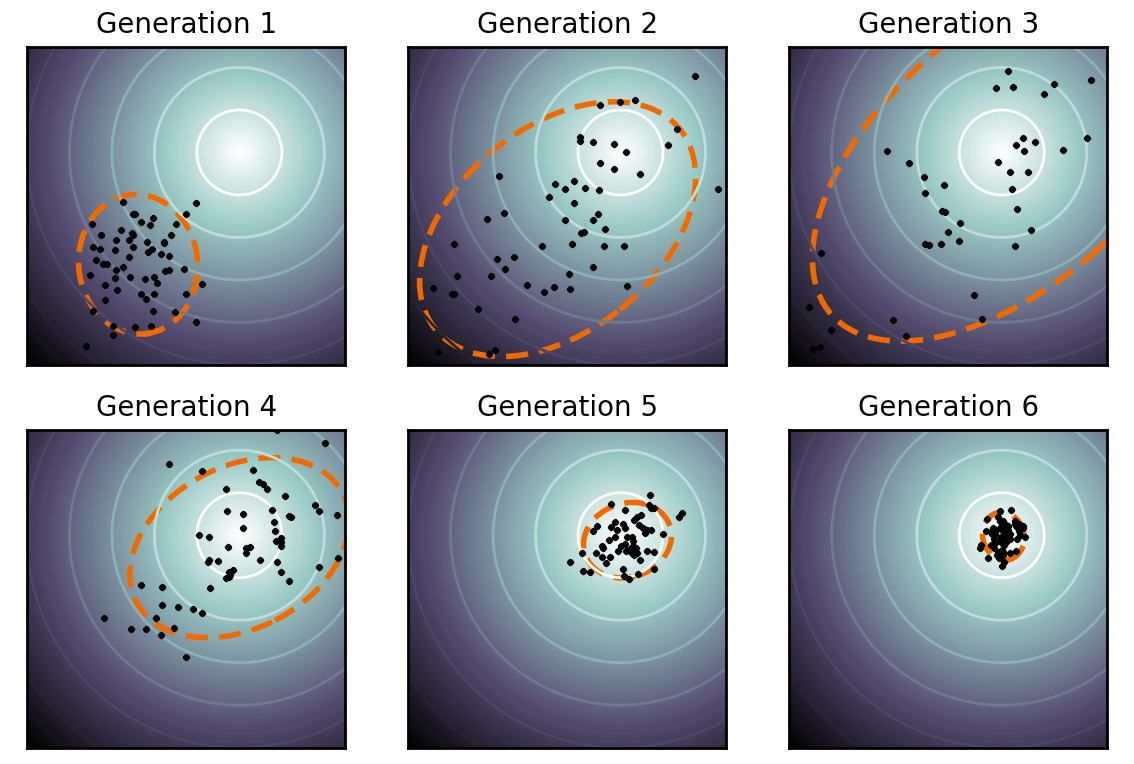
\includegraphics[width=0.6\textwidth, height=0.45\textheight]{figure_man/cmaes/cmaes_generations.png}
\end{figure}

\framebreak

\vspace{-30pt}
\begin{eqnarray*}
\xv^{[t+1](k)} \sim \bm{m}^{[t]} + \sigma^{[t]} \normal (\bm{0}, \bm{C}^{[t]}) \quad \text{for } k = 1, \dots, \lambda
\end{eqnarray*}

\begin{itemize}
\item $\xv^{[t+1](k)} \in \R^d$ is the $k$-th offspring (search point, individual) from generation $t+1$.
\item $\lambda \geq 2$ is the population/sample size, number of offsprings.
\end{itemize}

At generation $t$:

\begin{itemize}
\item $\normal(\bm{0}, \bm{C}^{[t]})$ is multivariate normal distribution with zero mean, covariance matrix $\bm{C}^{[t]}$. \textit{Note}: $\bm{m}^{[t]} + \sigma^{[t]} \normal(\bm{0}, \bm{C}^{[t]}) \sim \normal(\bm{m}^{[t]}, (\sigma^{[t]})^2 \bm{C}^{[t]})$.
\item $\bm{m}^{[t]} \in \R^d$ is the mean value of the search distribution.
\item $\sigma^{[t]} \in \R_{+}$ is the \enquote{overall} standard deviation/step size.
\item $\bm{C}^{[t]} \in \R^{d \times d}$ is the covariance matrix.
% Up to the scalar factor $\sigma^{(g)^2}$, $\bm{C}^{(g)}$ is the covariance matrix of the search distribution.
\end{itemize}

$\rightarrow$ \textit{How to calculate $\bm{m}^{[t+1]}$, $\bm{C}^{[t+1]}$, $\sigma^{[t+1]}$ for next generation $t+1$?}
\end{vbframe}


% \begin{vbframe}{Recall: Evolution Strategies (ES)}

% New search points are sampled normally distributed as perturbations of $\bm{m}$:
% \begin{eqnarray*}
% \xv_k \sim \bm{m} + \sigma \normal_k (\bm{0}, \bm{C}) \quad \text{for } k = 1, \dots, \lambda
% \end{eqnarray*}

% where $\xv_k$, $\bm{m} \in \R^{n}$, $\sigma \in \R_{+}$, $\bm{C} \in \R^{n \times n}$

% \begin{itemize}
% \item Mean vector $\bm{m} \in \R^d$ represents the favorite solution
% \item Step-size $\sigma \in \R_{+}$ controls the step length
% \item Covariance matrix $\bm{C} \in \R^{n \times n}$ determines the shape of the distribution ellipsoid.
% \end{itemize}

% Remaining question: How to update $\bm{m}$, $\bm{C}$ and $\sigma$?
% \end{vbframe}



% \begin{vbframe}{CMA-ES: Basic Method}
% \begin{enumerate}
% \item \textbf{Sample maximum entropy} distribution
% \item[] $x_i = m + \sigma \normal_i(\bm{0}, \bm{C})$ multivariate normal distribution
% \item \textbf{Ranking} solutions according to their fitness
% \item[] Invariance to order-preserving transformations
% \item \textbf{Update mean and covariance matrix} by natural gradient ascend, improving the \enquote{expected fitness} and the likelihood for good steps
% \item[] PCA $\rightarrow$ variable metric, new problem representation, invariant under changes of the coordinate system
% \item \textbf{Update step-size} based on non-local information
% \item[] Exploit correlations in the history of steps.
% \end{enumerate}
% \end{vbframe}



\begin{frame}
% \begin{eqnarray*}
% \bm{m} \leftarrow \bm{m} + \sigma \bm{y}_w, \quad \bm{y}_w = \sum_{i=1}^{\mu} w_i \bm{y}_{i:\lambda}, \quad \bm{y}_i\sim \normal_i(\bm{0}, \bm{C})
% \end{eqnarray*}

\begin{figure}
\begin{overprint}

\centering
\only<1>{
\frametitle{CMA-ES: Basic Method - Iteration 1}
\begin{enumerate}
\item \textbf{Sample} from distribution
\item[] $\xv^{[1](k)} = \bm{m}^{[0]} + \sigma^{[0]} \normal(\bm{0}, \bm{C}^{[0]})$ multivariate normal distribution.
\item[]
\end{enumerate}

\scalebox{0.6}{\includegraphics[width=1.5\textwidth, height=0.75\textheight]{figure_man/cmaes/cmaes_rankone_1.png}}

Initial distribution $\normal^{[0]} \sim (\bm{0}, \bm{\I}_2)$  of generation $t=0$.
}

\only<2>{
\frametitle{CMA-ES: Basic Method - Iteration 1}
\begin{enumerate}
\item \textbf{Sample} from distribution
\item[] $\xv^{[1](k)} = \bm{m}^{[0]} + \sigma^{[0]} \normal(\bm{0}, \bm{C}^{[0]})$ multivariate normal distribution.
\item[]
\end{enumerate}

\scalebox{0.6}{\includegraphics[width=1.5\textwidth, height=0.75\textheight]{figure_man/cmaes/cmaes_rankone_2.png}}

Initial distribution $\normal^{[0]} \sim (\bm{0}, \bm{\I}_2)$  of generation $t=0$, $\lambda = 6$.
}

\only<3>{
\frametitle{CMA-ES: Basic Method - Iteration 1}
\begin{enumerate}
\addtocounter{enumi}{1}
\item \textbf{Ranking} solutions according to their fitness (\textit{Selection} of $\mu$ best)
\item[] $\xv_{i:\lambda}$ as $i$-th ranked solution point, such that $f(\xv_{1:\lambda}) \leq \dots \leq f(\xv_{\lambda:\lambda})$.
\item[]
\end{enumerate}

\scalebox{0.6}{\includegraphics[width=1.5\textwidth, height=0.75\textheight]{figure_man/cmaes/cmaes_rankone_3.png}}

Calculation of auxiliary variable $\bm{y}_w := \sum_{i=1}^{\mu} w_i \xv_{i:\lambda}$, using $\mu = 3$ selected points (high fitness $\rightarrow$ high weights)

%Movement to new population mean $\bm{m}^{[1]}$ (disregarding $\sigma$) of the $\mu = 3$ selected points (high fitness $\rightarrow$ high weights, $\bm{y}_w := \sum_{i=1}^{\mu} w_i \xv_{i:\lambda}$).
}

\only<4>{
\frametitle{CMA-ES: Basic Method - Iteration 1}
\begin{enumerate}
\addtocounter{enumi}{2}
\item \textbf{Update covariance matrix} (\textit{Recombination}),
\item[] improving \enquote{expected fitness} and likelihood for good steps.
\item[]
\end{enumerate}

\scalebox{0.6}{\includegraphics[width=1.5\textwidth, height=0.75\textheight]{figure_man/cmaes/cmaes_rankone_4.png}}

Blue circle as a mixture of $\bm{C}$ and step $\bm{y}_w$ (simplified): $\bm{C}^{[1]} = 0.8 \bm{C}^{[0]} + 0.2 \bm{y}_w^{[0]} (\bm{y}_w^{[0]})^\top$ (Rank 1 update).
}

\only<5>{
\frametitle{CMA-ES: Basic Method - Iteration 1}
\begin{enumerate}
\addtocounter{enumi}{3}
\item \textbf{Update mean}
\item[]
\item[]
\end{enumerate}

\scalebox{0.6}{\includegraphics[width=1.5\textwidth, height=0.75\textheight]{figure_man/cmaes/cmaes_rankone_5.png}}

Movement towards the new distribution with mean $
\bm{m}^{[1]} = \bm{m}^{[0]} + \sigma^{[0]} \bm{y}_{w}^{[0]}$.
}

\only<6>{
\frametitle{CMA-ES: Basic Method - Iteration 2}
\begin{enumerate}
\item \textbf{Sample} from distribution for new generation
\item[] %(\textit{Mutation}) with $\xv^{[2](k)} = \bm{m}^{[1]} + \sigma^{[1]} \normal(\bm{0}, \bm{C}^{[1]})$ form multivariate
\item[] %normal distribution.
\end{enumerate}

\scalebox{0.6}{\includegraphics[width=1.5\textwidth, height=0.75\textheight]{figure_man/cmaes/cmaes_rankone_6.png}}

%New Distribution $\normal^{[1]}\sim (\bm{m}^{[1]}, \bm{C}^{[1]})$ (disregarding $\sigma$) \\
%of generation $t=1$, $\lambda = 6$.
}

\only<7>{
\frametitle{CMA-ES: Basic Method - Iteration 2}
\begin{enumerate}
\addtocounter{enumi}{1}
\item \textbf{Ranking} solutions according to their fitness (\textit{Selection} of $\mu$ best)
\item[] %$\xv_{i:\lambda}$ as $i$-th ranked solution point, such that $f(\xv_{1:\lambda}) \leq \dots \leq f(\xv_{\lambda:\lambda})$.
\item[]
\end{enumerate}

\scalebox{0.6}{\includegraphics[width=1.5\textwidth, height=0.75\textheight]{figure_man/cmaes/cmaes_rankone_7.png}}

%Movement to new population mean $\bm{m}^{[2]}$ (disregarding $\sigma$) of the $\mu = 3$ selected points (high fitness $\rightarrow$ high weights, $\bm{y}_w := \sum_{i=1}^{\mu} w_i \xv_{i:\lambda}$).
}

\only<8>{
\frametitle{CMA-ES: Basic Method - Iteration 2}
\begin{enumerate}
\addtocounter{enumi}{2}
\item \textbf{Update mean and covariance matrix} (\textit{Recombination})
\item[] %improving \enquote{expected fitness} and likelihood for good steps.
\item[]
\end{enumerate}

\scalebox{0.6}{\includegraphics[width=1.5\textwidth, height=0.75\textheight]{figure_man/cmaes/cmaes_rankone_8.png}}

%Blue circle as a mixture of $\bm{C}$ and step $\bm{y}_w$: $\bm{C}^{[2]} \leftarrow 0.8 \bm{C}^{[1]} + 0.2  \bm{y}_w^{[1]} (\bm{y}_w^{[1]})^\top$.
}

\only<9>{
\frametitle{CMA-ES: Basic Method - Iteration 2}
\begin{enumerate}
\addtocounter{enumi}{3}
\item \textbf{Update step-size} based on non-local information,
\item[] exploit correlations in the history of steps.
\item[]
\end{enumerate}

\scalebox{0.6}{\includegraphics[width=1.5\textwidth, height=0.75\textheight]{figure_man/cmaes/cmaes_rankone_9.png}}

%Movement towards the new distribution (disregarding $\sigma$) with mean $
%\bm{m}^{[2]} = \bm{m}^{[1]} + \sigma^{[1]} \bm{y}_{w}^{[1]}$.
}
\end{overprint}
\end{figure}
\end{frame}



%\begin{vbframe}{Updating \MakeLowercase{$\bm{m}$}: The $(\mu/\mu_W, \lambda)$-ES}
%
%$(\mu/\mu_W, \lambda)$-ES marks the \textbf{E}volution \textbf{S}trategy with $\bm{\mu}$ parents, \textbf{W}eighted recombination of all $\bm{\mu}$ parents and $\bm{\lambda}$ offspring.
%
%\lz
%
%Let $\xv_{i:\lambda}$ be the $i$-th ranked solution point, the new mean vector is
%% such that $f(\xv_{1:\lambda}) \leq \dots \leq f(\xv_{\lambda:\lambda})$.
%
%\vspace{-10pt}
%\begin{eqnarray*}
%\bm{m}^{[t+1]} = \bm{m}^{[t]} + \sigma^{[t]} \underbrace{\sum_{i=1}^{\mu} w_i \xv_{i:\lambda}^{[t]}}_{=: \bm{y}_w^{[t]}}
%\end{eqnarray*}
%
%where $w_1 \geq \dots \geq w_{\mu} > 0$, $\sum_{i=1}^{\mu} w_i = 1$ and $\frac{1}{\sum_{i=1}^{\mu} w_i^2} =: \mu_w \approx \frac{\lambda}{4}$.
%
%\lz
%
%The best $\mu$ points are selected from the new solutions (non-elitistic) and weighted intermediate recombination is applied.
%
%\lz
%
%If $w_{i=1:\mu} = 1/\mu$ then $\bm{y}_w$ is equal to the mean of the $\mu$ best points.
%\end{vbframe}


%\begin{vbframe}{Updating \MakeLowercase{$\bm{m}$}: The $(\mu/\mu_W, \lambda)$-ES}
%
%Remarks on weights $w_i$
%
%\begin{itemize}
%\item $w_{i=1:\mu} \in \R_{>0}$ are positive weight coefficients for recombination
%\item Typically chosen as weighted average of $\mu$ selected points $w_{i=1:\mu} = 1/\mu$
%\item Assigning different weights $w_i$ should be interpreted as a selection mechanism
%\item Approaches exist, which give the remaining $\lambda-\mu$ points negative weights, such that $\lambda$ weights in total are used (e.g active covariance matrix adaptation)
%\item Weights depend only on the ranking, not on the function values directly $\rightarrow$ renders the algorithm invariant under order-preserving transformation of the objective function
%\end{itemize}
%\end{vbframe}


\begin{vbframe}{Updating $C$: CMA - Rank-One Update}
Initialize $\bm{m} \in \R^d$ and $\bm{C} = \bm{\I}$, set $\sigma = 1$, learning rate $c_{cov} \approx 2/d^2$. While not terminate

\begin{align*}
\xv^{(k)} &= \bm{m} + \sigma \normal_i(\bm{0}, \bm{C}) \\
\bm{m} &\leftarrow \bm{m} + \sigma \bm{y}_w, \quad \text{where } \bm{y}_w = \sum_{i=1}^\mu \bm{w}_i\xv_{i:\lambda} \\
\bm{C} &\leftarrow (1-c_{cov}) \bm{C} + c_{cov}\mu_w \underbrace{\bm{y}_w\bm{y}_w^\top}_{\text{rank-one}}, \quad \text{where } \mu_w = \frac{1}{\sum_{i=1}^\mu w_i^2}
\end{align*}

The rank-one update was developed in several domains independently, conducting a \textbf{principle component analysis} (PCA) of steps $\bm{y}_w$ sequentially in time and space.

\lz

\textit{In principle}: the adaptation increases the likelihood of successful steps $\bm{y}_w$ to appear again.

% \textit{Different viewpoint}: the adaptation follows a natural gradient approximation of the expected fitness.

% \framebreak

% \begin{eqnarray*}
% \bm{C} &\leftarrow (1-c_{cov}) \bm{C} + c_{cov}\mu_w \bm{y}_w\bm{y}_w^\top
% \end{eqnarray*}

% \begin{itemize}
% \item Conducting a \textbf{principle component analysis} (PCA) of steps $\bm{y}_w$ sequentially in time and space
% \item Approximation of the \textbf{inverse Hessian} on quadratic functions
% \item Learning of a new \textbf{rotated problem representation}
% \item[] Components only independent in the new representation
% \item Learning of all \textbf{pairwise dependencies} between variables
% \item[] Dependencies reflected by off-diagonal entries in the covariance matrix
% \item Learning of a \textbf{new} (Mahalanobis) \textbf{metric}
% \item For $\mu = 1$: Conducting a \textbf{natural gradient ascent} on the normal distribution $\normal$ (independent of the given coordinate system).
% \end{itemize}

\end{vbframe}

%\begin{vbframe}{Updating $C$: CMA - Cumulation}
%\enquote{Cumulation} as a widely used technique and known under various names (\textit{exponential smoothing} in forecasting and time series, exponentially weighted \textit{moving average}, \textit{iterate averaging} in stochastic approximation, etc.).
%
%\lz
%
%Using cumulation / an evolution path for the rank-one update of the covariance matrix reduces the number of function evaluations to adapt to a straight ridge from about $\order(d^2)$ to $\order(d)$.
%
%\lz
%
%For the evolution/search path taken over a number of generation steps an exponentially weighted sum of steps $\bm{y}_w$ is used:
%
%\begin{eqnarray*}
%\bm{p}_c \propto \sum_{t = 0}^T \underbrace{(1-c_{\bm{c}})^{T-i}}_{\substack{\text{exponentially} \\ \text{fading weights}}} \bm{y}_w^{[t]}
%\end{eqnarray*}
%
%\framebreak
%
%Cumulation as \textit{recursive construction of the evolution path}:
%
%\begin{eqnarray*}
%\bm{p}_c^{[t+1]} = \underbrace{(1- c_{\bm{c}})}_{\text{decay factor}} \bm{p}_c^{[t]} + \underbrace{\sqrt{1-(1-c_{\bm{c}})^2}}_{\text{normalization factor}} \sqrt{\mu_w} \underbrace{\bm{y}_w^{[t]}}_{input},
%\end{eqnarray*}
%
%where $\bm{y}_{w}^{[t]} = \frac{\bm{m}^{[t+1]} - \bm{m}^{[t]}}{\sigma^{[t]}}$ and $\mu_w = \frac{1}{\sum w_i^2}$, $c_{C} << 1$. %FIXME: \ll
%History information is accumulated in the evolution path.
%
%\begin{figure}
%  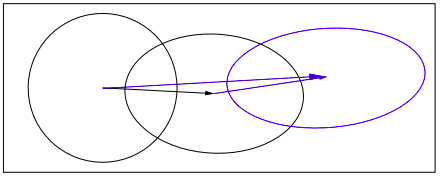
\includegraphics[width=0.8\textwidth, height=0.4\textheight]{figure_man/cmaes/cmaes_cumulation_1.png}
%\end{figure}
%
%\framebreak
%
%
%$\bm{y}_w \bm{y}_w^\top$ was used for updating $\bm{C}$ and because $\bm{y}_w \bm{y}_w^\top = -\bm{y}_w (-\bm{y}_w)^\top$ the sign of $\bm{y}_w$ is lost.
%
%\lz
%
%The \textbf{sign information} (signifying correlation between steps) is (re-)introduced by using the \textit{evolution path}.
%
%\begin{align*}
%\bm{p}_c^{[t+1]} &= \underbrace{(1- c_{\bm{c}})}_{\text{decay factor}} \bm{p}_{\bm{c}}^{[t]} + \underbrace{\sqrt{1-(1-c_{\bm{c}})^2}}_{\text{normalization factor}} \sqrt{\mu_w} \bm{y}_w^{[t]} \\
%\bm{C}^{[t+1]} &= (1- c_{cov}) \bm{C}^{[t]} + c_{cov} \underbrace{\bm{p}_c^{[t+1]} (\bm{p}_c^{[t+1]})^\top}_{\text{rank-one}},
%\end{align*}
%
%where $\mu_w = \frac{1}{\sum w_i^2}, c_{cov} << c_{\bm{C}} << 1$, such that $1/{c_{\bm{c}}}$ is the \enquote{backward time horizon}. %FIXME: \ll
%
%\framebreak
%
%\begin{align*}
%\textcolor{green}{\bm{p}_c^{[t+1]}} &= \underbrace{(1- \textcolor{blue}{c_{\bm{c}}})}_{\text{decay factor}} \textcolor{green}{\bm{p}_{\bm{c}}^{[t]}} + \underbrace{\sqrt{1-(1-\textcolor{blue}{c_{\bm{c}}})^2}}_{\text{normalization factor}} \sqrt{\mu_w} \bm{y}_w^{[t]} \\
%\textcolor{green}{\bm{C}^{[t+1]}} &= (1- \textcolor{blue}{c_{cov}})\textcolor{green}{\bm{C}^{[t]}} + \textcolor{blue}{c_{cov}} \underbrace{\textcolor{green}{\bm{p}_c^{[t+1]} (\bm{p}_c^{[t+1]}})^\top}_{\text{rank-one}},
%\end{align*}
%\vspace{-10pt}
%
%where $\mu_w = \frac{1}{\sum \textcolor{blue}{w_i}^2}, \textcolor{blue}{c_{cov}} << \textcolor{blue}{c_{\bm{C}}} << 1$, such that $1/{c_{\bm{c}}}$ is the \enquote{backward time horizon}. %FIXME: \ll
%
%\begin{figure}
%  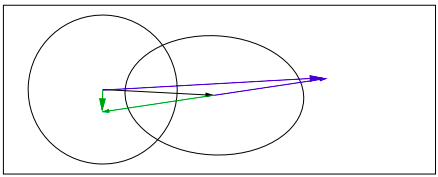
\includegraphics[width=0.8\textwidth, height=0.37\textheight]{figure_man/cmaes/cmaes_cumulation_2.png}
%\end{figure}
%
%\end{vbframe}

%
%\begin{vbframe}{Updating $C$: CMA - Rank-$\mu$ Update}
%In case of \textit{large population sizes $\lambda$} the \textbf{rank-$\mu$ update} extends the update rule using $\mu > 1$ vectors to update$\bm{C}$ at each generation step.
%
%\lz
%
%The weighted empirical covariance matrix computes a weighted mean of the outer products of the best $\mu$ steps and has rank $\min(\mu, d)$ with probability 1.
%
%\vspace{-10pt}
%
%\begin{eqnarray*}
%\bm{C}_\mu^{[t+1]} = \sum_{i=1}^\mu \bm{w}_i \xv_{i:\lambda}^{[t+1]} (\xv_{i:\lambda}^{[t+1]})^\top
%\end{eqnarray*}
%
%The rank-$\mu$-update then reads
%\begin{eqnarray*}
%\bm{C}^{[t+1]} = (1-c_{cov}) \bm{C}^{[t]} + c_{cov} \bm{C}_{\mu}^{[t+1]},
%\end{eqnarray*}
%
%where $c_{cov} \approx \mu_w/d^2$ and $c_{cov} \leq 1$.
%
%\framebreak
%
%\begin{figure}
%  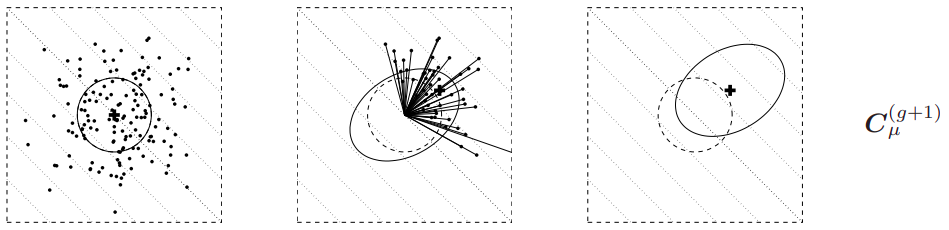
\includegraphics[width=1\textwidth, height=0.3\textheight]{figure_man/cmaes/cmaes_rankmu.png}
%\end{figure}
%
%\begin{enumerate}
%  \item Sampling $\lambda = 150$ solutions, where $\bm{C}^{[t]} = \bm{\I}$ and $\sigma^{[t]} = 1$.
%  \item[] $\xv^{[t+1](k)} = \bm{m}^{[t]} + \sigma^{[t]} \normal(\bm{0}, \bm{C}^{[t]})$
%  \item Calculation $\bm{C}$, where $\mu = 50$, $w_1 = \dots = w_{\mu} = 1/\mu$ and $c_{cov}=1$
%  \item[] $\bm{C}_{\mu}^{[t+1]} = 1/\mu \sum \xv_{1:\lambda}^{[t]} (\xv_{1:\lambda}^{[t]})^\top$ and $\bm{C}^{[t+1]} = (1-1) \times \bm{C}^{[t]} + 1 \times \bm{C}_{\mu}^{[t+1]}$
%  \item New distribution
%  \item[] $\bm{m}^{[t+1]} = \bm{m}^{[t]} + 1/\mu \sum \xv_{1:\lambda}^{[t]}$.
%\end{enumerate}
%
%\end{vbframe}
%
%
%\begin{vbframe}{Updating $C$: Rank-One and Rank-$\mu$ Update}
%\textbf{Rank-one update}
%
%\begin{itemize}
%\item Uses the evolution path
%\item Can reduce the number of \textit{function evaluations} to adapt to straight ridges from about $\order(d^2)$ to $\order(d)$.
%\end{itemize}
%
%\textbf{Rank-$\mu$ update}
%
%\begin{itemize}
%\item Increases the learning rate in large populations and therefore the primary mechanism for large populations (thumb rule: $\lambda \geq 3d + 10$)
%\item Can reduce the number of \textit{generations} from about $\order(d^2)$ to $\order(d)^{(12)}$, given $\mu_w\propto \lambda \propto d$.
%\end{itemize}
%
%
%\textbf{Hybrid Update}: rank-one and rank-$\mu$ update can be combined.
%\end{vbframe}



\begin{vbframe}{Updating $\sigma$: Methods Step-Size Control}
\begin{itemize}
\item \textbf{$1/5$-th success rule}: increases the step-size if more than 20 \% of the new solutions are successful, decrease otherwise
\item \textbf{$\sigma$-self-adaptation}: mutation is applied to the step-size and the better - according to the objective function value - is selected
\item \textbf{Path length control via cumulative step-size adaptation (CSA)}: self-adaptation derandomized and non-localized
\item Alternative step-size adaptation mechanism: two-point step-size adaptation, median success rule, population success rule.
\end{itemize}
\end{vbframe}

%\begin{vbframe}{Updating $\sigma$: Path Length Control (CSA)}
%Measure the length of the evolution path with informal steps:
%\begin{itemize}
%\item perpendicular under random selection (in expectation)
%\item perpendicular in the desired solution (to be most effective)
%\end{itemize}
%
%\begin{figure}
%  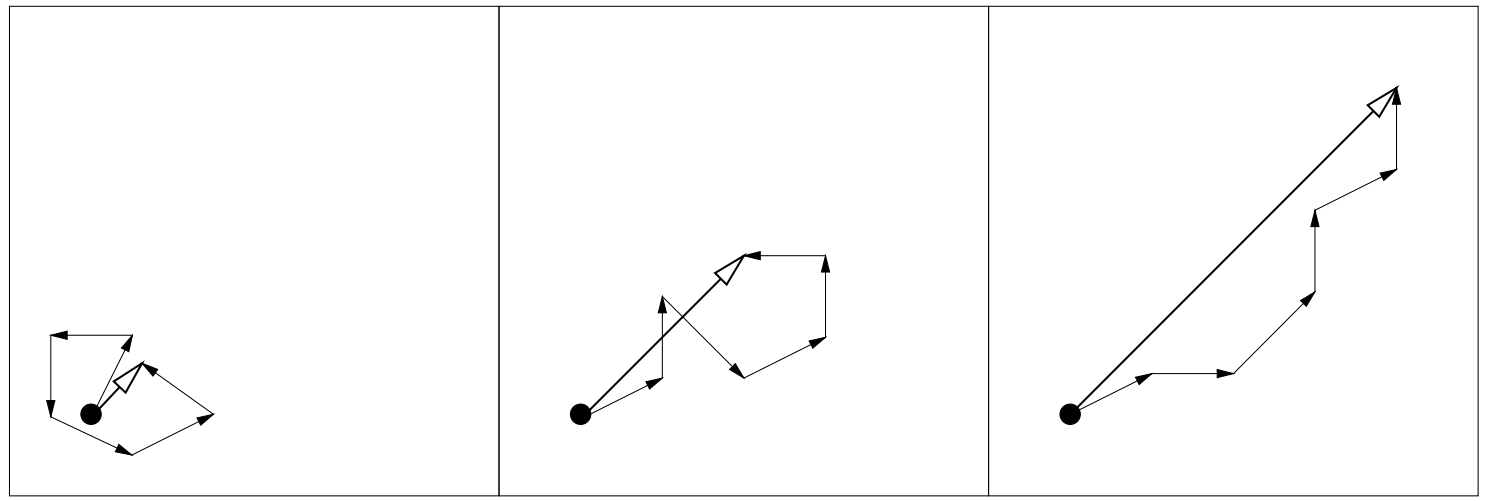
\includegraphics[width=1\textwidth, height=0.33\textheight]{figure_man/cmaes/cmaes_path.png}
%\end{figure}
%
%Pathway of mean vector $\bm{m}$ in the generation sequence of above pictures
%\begin{enumerate}
%\item decreases $\sigma$ as single steps cancel each other off
%\item ideal case as single steps are uncorrelated
%\item increases $\sigma$ as single steps point in same direction
%\end{enumerate}
%
%\framebreak
%
%Initialize $\bm{m} \in \R^d$, $\sigma \in \R_+$, evolution path $p_\sigma = \bm{0}$.
%
%Set $c_\sigma \approx 4/d$, $d_\sigma \approx 1$.
%
%\begin{align*}
%\bm{m}^{[t+1]} &= \bm{m}^{[t]} + \sigma^{[t]} \bm{y}_w^{[t]}\\
%\bm{p}_\sigma^{[t+1]} &= (1- c_\sigma) \bm{p}_\sigma^{[t]} + \underbrace{\sqrt{1-(1-c_\sigma)^2}}_{\text{accounts for } 1-c_\sigma} \underbrace{\sqrt{\mu_w}}_{\text{account for} w_i} \bm{y}_w^{[t]} \\
%\sigma^{[t+1]} &= \sigma^{[t]} \times \underbrace{\exp\biggl( \frac{c_\sigma}{d_\sigma}\Bigl(\frac{||\bm{p}_\sigma^{[t+1]}||}{\E||\normal(\bm{0}, \bm{\I})||} - 1 \Bigl)\biggl)}_{>1 \Longleftrightarrow ||\bm{p}_\sigma|| \text{ is greater than its expectation}}
%\end{align*}
%
%\framebreak
\begin{vbframe}{Updating $\sigma$: Path Length Control (CSA)}
\begin{figure}
  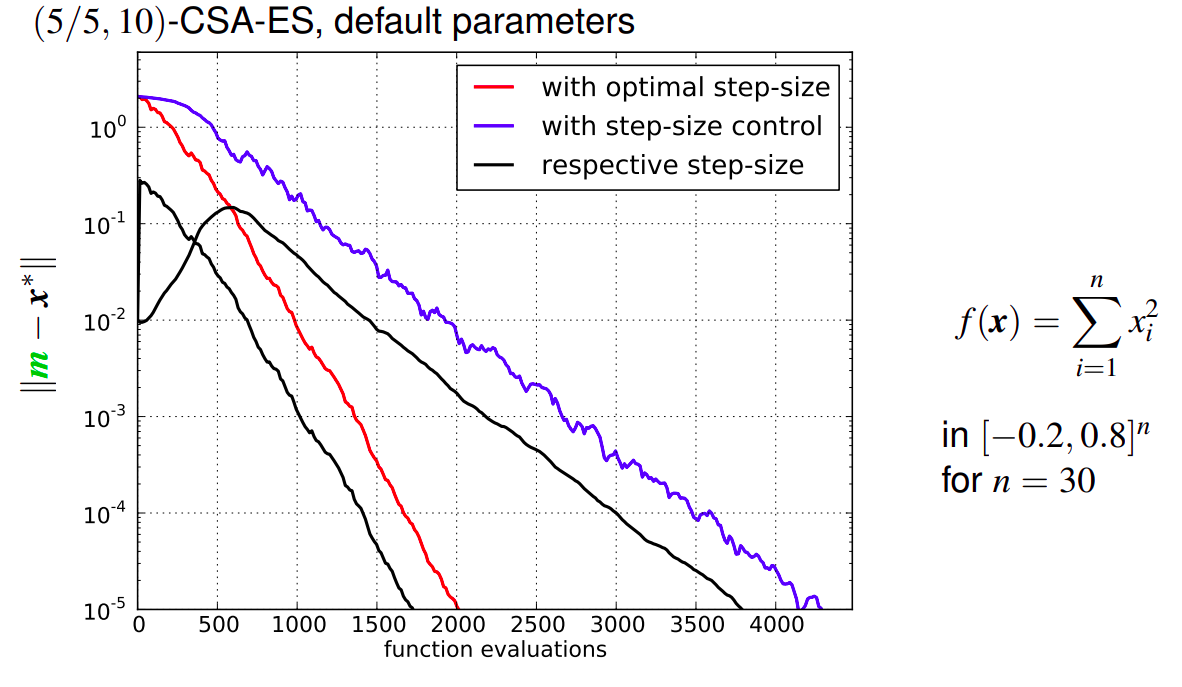
\includegraphics[width=1\textwidth, height=0.7\textheight]{figure_man/cmaes/cmaes_step-size.png}
\end{figure}

CSA effective and robust for $\lambda \leq N$.

\end{vbframe}


% \begin{frame}{Updating $C$: CMA - Rank-One Update}
% \begin{eqnarray*}
% \bm{m} \leftarrow \bm{m} + \sigma \bm{y}_w, \quad \bm{y}_w = \sum_{i=1}^{\mu} w_i \bm{y}_{i:\lambda}, \quad \bm{y}_i\sim \normal_i(\bm{0}, \bm{C})
% \end{eqnarray*}

% \begin{figure}
% \begin{overprint}
% \centering
% \only<1>{\scalebox{0.6}{\includegraphics[width=1.5\textwidth, height=0.75\textheight]{figure_man/cmaes_rankone_1.png}}

% Initial distribution with $\bm{C} = 1$.}
% \only<2>{\scalebox{0.6}{\includegraphics[width=1.5\textwidth, height=0.75\textheight]{figure_man/cmaes_rankone_2.png}}

% Initial distribution with $\bm{C} = 1$.}
% \only<3>{\scalebox{0.6}{\includegraphics[width=1.5\textwidth, height=0.75\textheight]{figure_man/cmaes_rankone_3.png}}

% Movement to the population mean $m$ (disregarding $\sigma$) with $\bm{y}_w$.}
% \only<4>{\scalebox{0.6}{\includegraphics[width=1.5\textwidth, height=0.75\textheight]{figure_man/cmaes_rankone_4.png}}

% Blue circle as a mixture of $\bm{C}$ and step $\bm{y}_w$: $\bm{C} \leftarrow 0.8\times \bm{C} + 0.2 \times \bm{y}_w \bm{y}^\top$.}
% \only<5>{\scalebox{0.6}{\includegraphics[width=1.5\textwidth, height=0.75\textheight]{figure_man/cmaes_rankone_5.png}}

% Movement towards the new distribution (disregarding $\sigma$).}
% \only<6>{\scalebox{0.6}{\includegraphics[width=1.5\textwidth, height=0.75\textheight]{figure_man/cmaes_rankone_6.png}}

% New Distribution (disregarding $\sigma$).}
% \only<7>{\scalebox{0.6}{\includegraphics[width=1.5\textwidth, height=0.75\textheight]{figure_man/cmaes_rankone_7.png}}

% Movement to the population mean $\bm{m}$.}
% \only<8>{\scalebox{0.6}{\includegraphics[width=1.5\textwidth, height=0.75\textheight]{figure_man/cmaes_rankone_8.png}}

% Green circle as a mixture of $\bm{C}$ and step $\bm{y}_w$: $\bm{C} \leftarrow 0.8\times \bm{C} + 0.2 \times \bm{y}_w \bm{y}^\top$.}
% \only<9>{\scalebox{0.6}{\includegraphics[width=1.5\textwidth, height=0.75\textheight]{figure_man/cmaes_rankone_9.png}}

% Movement towards the new distribution (disregarding $\sigma$).}
% \end{overprint}
% \end{figure}
% \end{frame}


\endlecture
\end{document}

